\documentclass[12pt]{article}

\usepackage[utf8]{inputenc}
\usepackage[english]{babel}
\usepackage{sectsty}
\usepackage{multicol, caption}
\usepackage{graphicx}
\usepackage{wrapfig}
\usepackage{subfig}
\usepackage{hyperref}
%\usepackage{subcaption}

%\usepackage{biblatex}
\usepackage[margin=1.0in]{geometry} % don't know what size margins to use
\newenvironment{Figure}
  {\par\medskip\noindent\minipage{\linewidth}}
  {\endminipage\par\medskip}

\setlength{\columnsep}{1cm}

\sectionfont{\fontsize{12}{15}\selectfont}
\subsectionfont{\fontsize{12}{15}\selectfont}
 

\begin{document}
    \begin{center}
        \textbf{Evaluation of Classifiers and Feature Selection on Spam Filtering} 
    \end{center}

    \begin{center}
        Griffin Dunn and William Thompson
    \end{center}

    \textbf{Abstract:} 
        In this paper we explore the effects of extracting features that are not 
        solely based on word frequency and the selection of classifier for the task
        of determining if a message is spam or not spam (ham). These methods
        will be tested on a publicly available corpora and compared to the results
        of other models introduced by other authors. Classifiers will be selected
        from the variety available through the open-source Python module scikit-learn.

    \begin{multicols}{2}
        \section{Introduction}
            The classification of spam emails is an important task in today's society,
            as we receive potentially hundreds of them a year which clutter
            an already full inbox. These emails also pose a threat to the uninformed
            as many ask for personal information, such as street addresses and banking details.
            Traditionally emails have been filtered through rule-based systems that
            could be reverse engineered to still allow for spam email to get through.
            Some newer filters take advantage of machine learning techniques and use
            them in conjunction with the traditional method which leads to good results,
            but still some emails get through. Some newer classifiers may hold the
            key to filtering out even the most engineered emails.
            
            
            As machine learning has had a resurgence, a variety
            of new classifier algorithms and implementations have surfaced that 
            make it quick and easy to implement one of these systems. Along with this,
            an explosion of open-source libraries have made difficult parsing tasks
            such as handling raw email data trivial. With this boom, public corpora
            have been created through crowd sourcing, which allow individuals to
            test their ideas on realistic data.

            \begin{Figure}
                \centering
                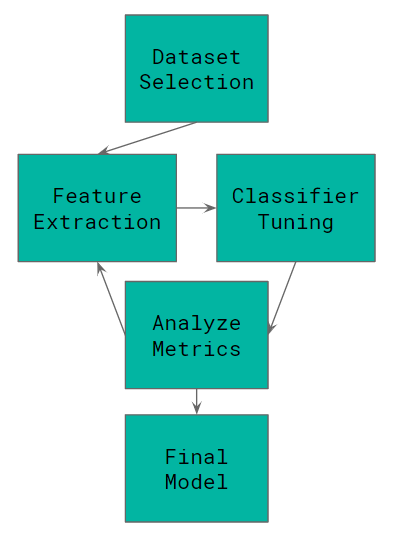
\includegraphics[width=\linewidth]{figures/process.png}
                \captionof{figure}{Our Machine Learning Process}\label{fig:process}
            \end{Figure}


            In this paper we explore the selection public datasets, data preparation,
            feature extraction and finally the selection and tuning of classifiers.
            We will do this following the process illustrated in \autoref{fig:process}.
        \section{Dataset Selection}
            The correct selection of a dataset was crucial to the testing of 
            different types of features. There were many characteristics that were
            on our `wishlist.' Such as having the freedom of processing 
            the raw text ourselves and determining what features may be important, 
            and not have the data preproccesed or turned into vectors.
            Next we wanted data that was conversational, that didn't use too much 
            slang or leetspeak and was in general proper English. The size of the
            dataset needed to be fairly large, at least 1000, for frequency analysis.
            Lastly, we would like a dataset that was referenced in multiple papers to make comparisons
            of our results to others. 
            
            So we shortlisted a few datasets that fulfilled some of these characteristics, but
            settled on the SpamAssasin Dataset which fulfilled all of our requirements
            with raw email data that mostly consisted of both business and casual
            conversations\cite{sa_dataset}. It consisted of both easy and hard data, but we stuck with
            just the easy data as many of the hard pieces of data were too difficult
            to classify without more information about the user.

        \section{Data Preparation}
            
            With so much metadata given with this dataset, we wanted to take advantage
            of it for use as potential features. In preprocessing we found many features
            that could signature of spam emails such as excessive links or attachments.
            The processes illustrated with \autoref{fig:preprocess}, is an overview
            of the processes that will be preformed in this step.


            \begin{Figure}
                \centering
                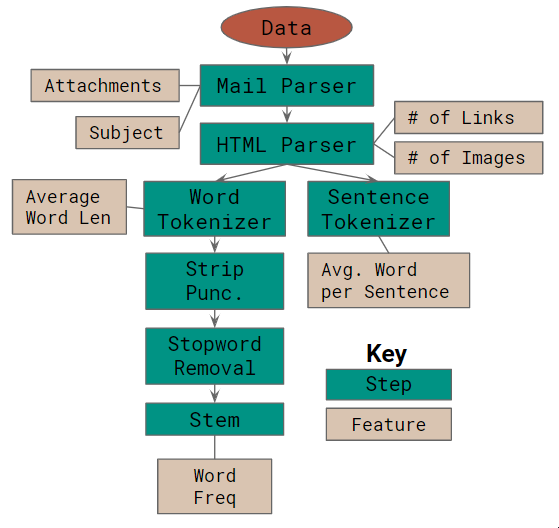
\includegraphics[width=\linewidth]{figures/prep.png}
                \captionof{figure}{Preparation Process}\label{fig:preprocess}
            \end{Figure}


            Once data was loaded in we started by running the data the data through
            the Python Standard Library's mail parser, which striped the mail headers
            and put them into a map for separate analysis. It also handled multi-part
            data as files were encoded into the file in base64, and allowed us to count
            the amount of attachments. Without using a mail
            parser it would be difficult to just get the body of the text which
            would be used for feature extraction. Other papers left this data in the
            email, possibly because this information is hard to extract and the tools
            weren't as easily accessible when their implementation was written. We
            decided to strip this data out as to not add noise and also because many 
            headers were left on from other spam checkers, identifying whether or not
            it believed the message was spam or ham.


            Next we used BeautifulSoup's HTML parser to interpret any HTML data that
            was in an email. We queried the document structure for the \textit{href}
            attribute because it indicates a link. Not only an \textit{a} tag can include
            a link, tags such as an \textit{img} tag can also contain one. Potential attackers
            may also use an \textit{a} tag to make a link look like it is going somewhere else,
            such as having the text \textit{http://google.com} a clickable link to
            \textit{http://mygooglephishingsite.com}, but we didn't see this practice 
            occurring in this dataset so we ignored this potential feature. We also looked at the
            amount of linked pictures, as an attacker may try to get credibility with it's prey
            by introducing fancy graphics. Lastly we extracted the raw content from the HTML,
            ignoring any structure that was present for tokenization.


            The tokenization step was done with NLTK's word and sentence tokenizer.
            The sentence tokens were used for some metrics such as average words per
            sentence and could be used in the future for the analysis of sentence
            structure. The word tokens were stripped of punctuation such as '.',
            '?', '(' and ')', which would litter our unigrams. Next we removed stopwords
            from the provided list of English stopwords in NLTK's corpus. Removing
            these words are necessary as they provide no direct meaning when it comes
            to frequency analysis of the documents and would just provide more noise
            in the classifier. Lastly we
            stemmed the words using NLTK's Porter Stemmer with their extensions to
            Martin Porter's algorithm. This allowed use to remove suffixes such as '-s',
            which would group `business' and `businesses' separately.


            Now data was stored in memory as Python objects for processing through the
            feature extractor. We shuffled and then split the data 
            80:20 into a training and testing set respectively.
        
        \section{Feature Extraction}

            The next step is to extract the necessary features and then vectorize
            them for training with our classifier. 
            
            \begin{Figure}
                \centering
                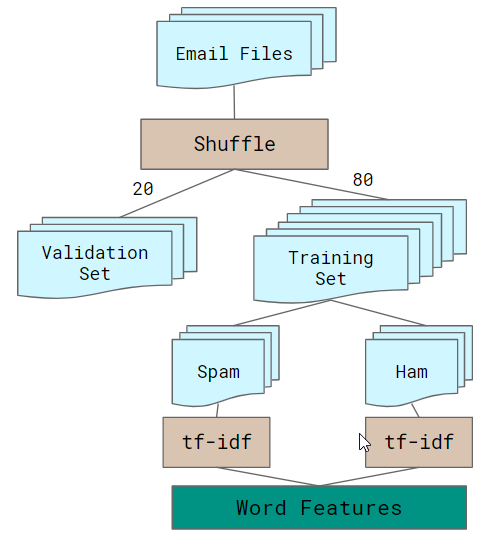
\includegraphics[scale=0.5]{figures/extract.png}
                \captionof{figure}{Extraction Process}
                \label{fig:extrac}
            \end{Figure}
            
            
            The first step of extraction was
            to find words that meant the most to the corpus which we defined as
            the body of the email. To accomplish this
            we used the tf-idf algorithm implemented in scikit-learn. This algorithm helps
            weigh down words that are too common, and bring up words that are important
            to the corpus. Next we split the documents into spam and ham before analysis.
            This was done because this algorithm is still based on frequency and the
            ratio of ham to spam was not 1:1. Characteristic words to spam emails such
            as ``free'' wouldn't show up because they're not prominent in ham emails.

            \begin{minipage}{0.4\columnwidth}
                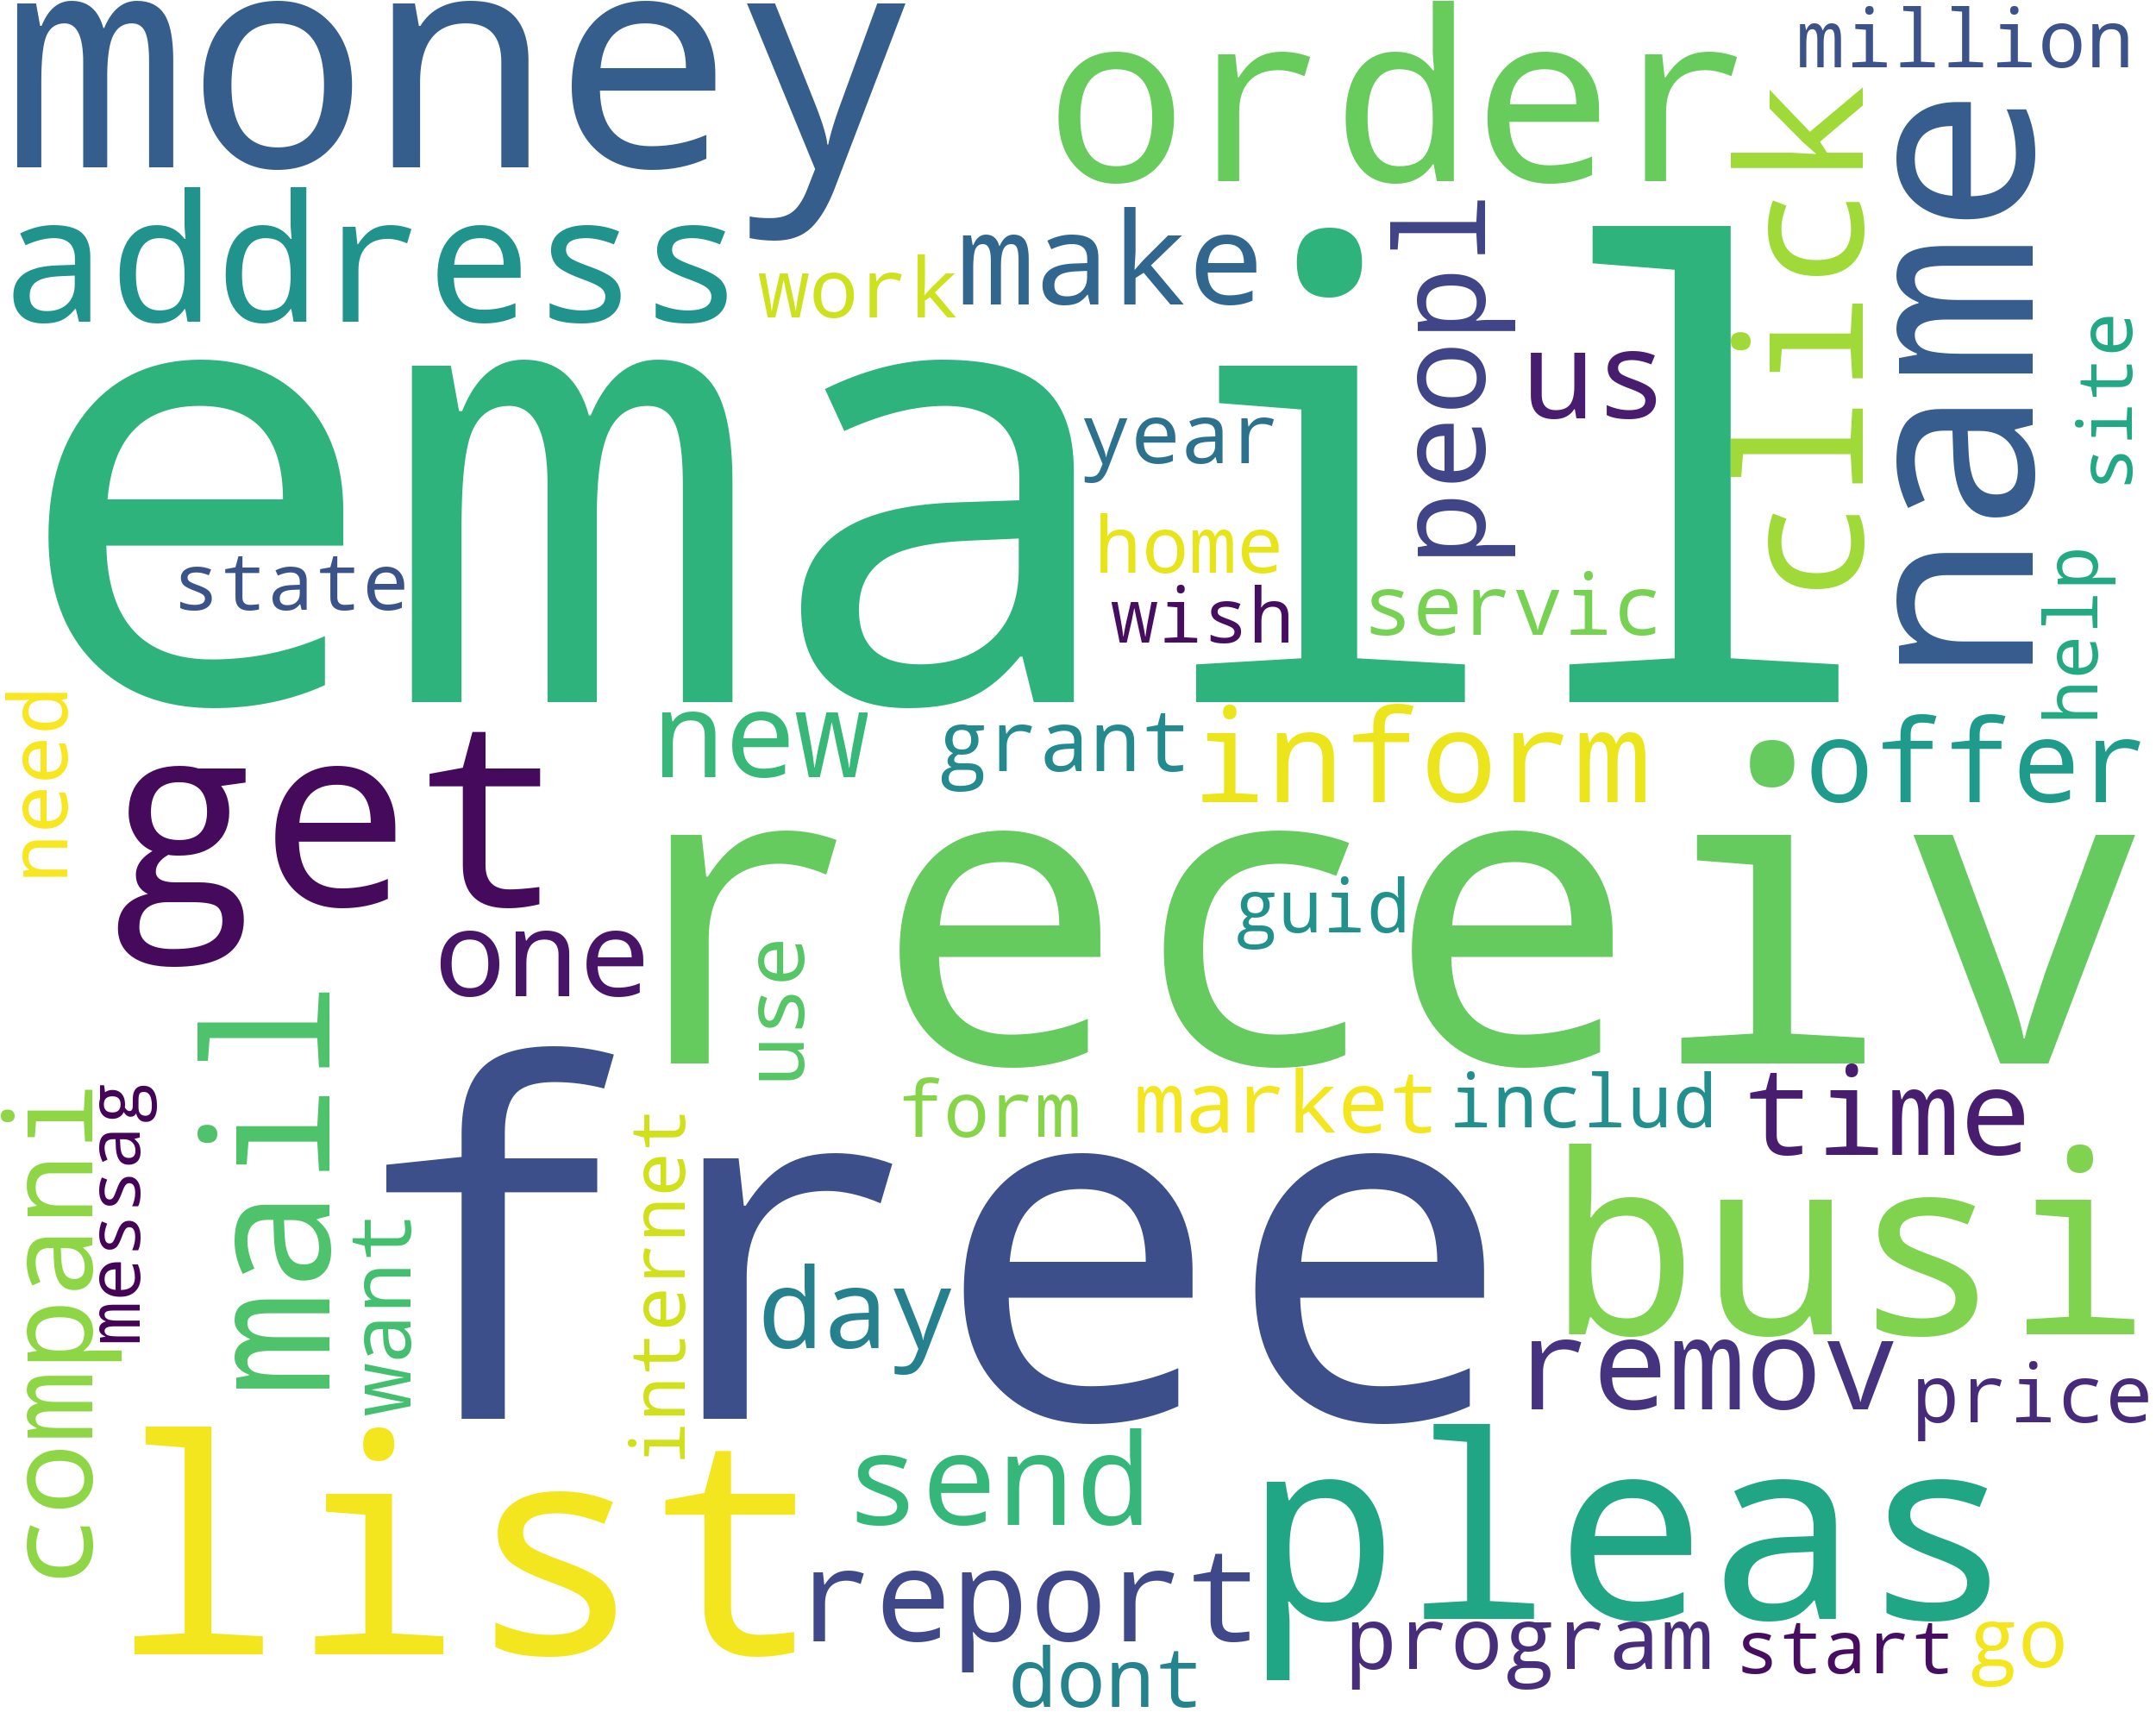
\includegraphics[width=\textwidth]{figures/spam_wc}
                \captionof{figure}{Spam}\label{fig:spam_wc}
            \end{minipage}
            \begin{minipage}{0.4\columnwidth}
                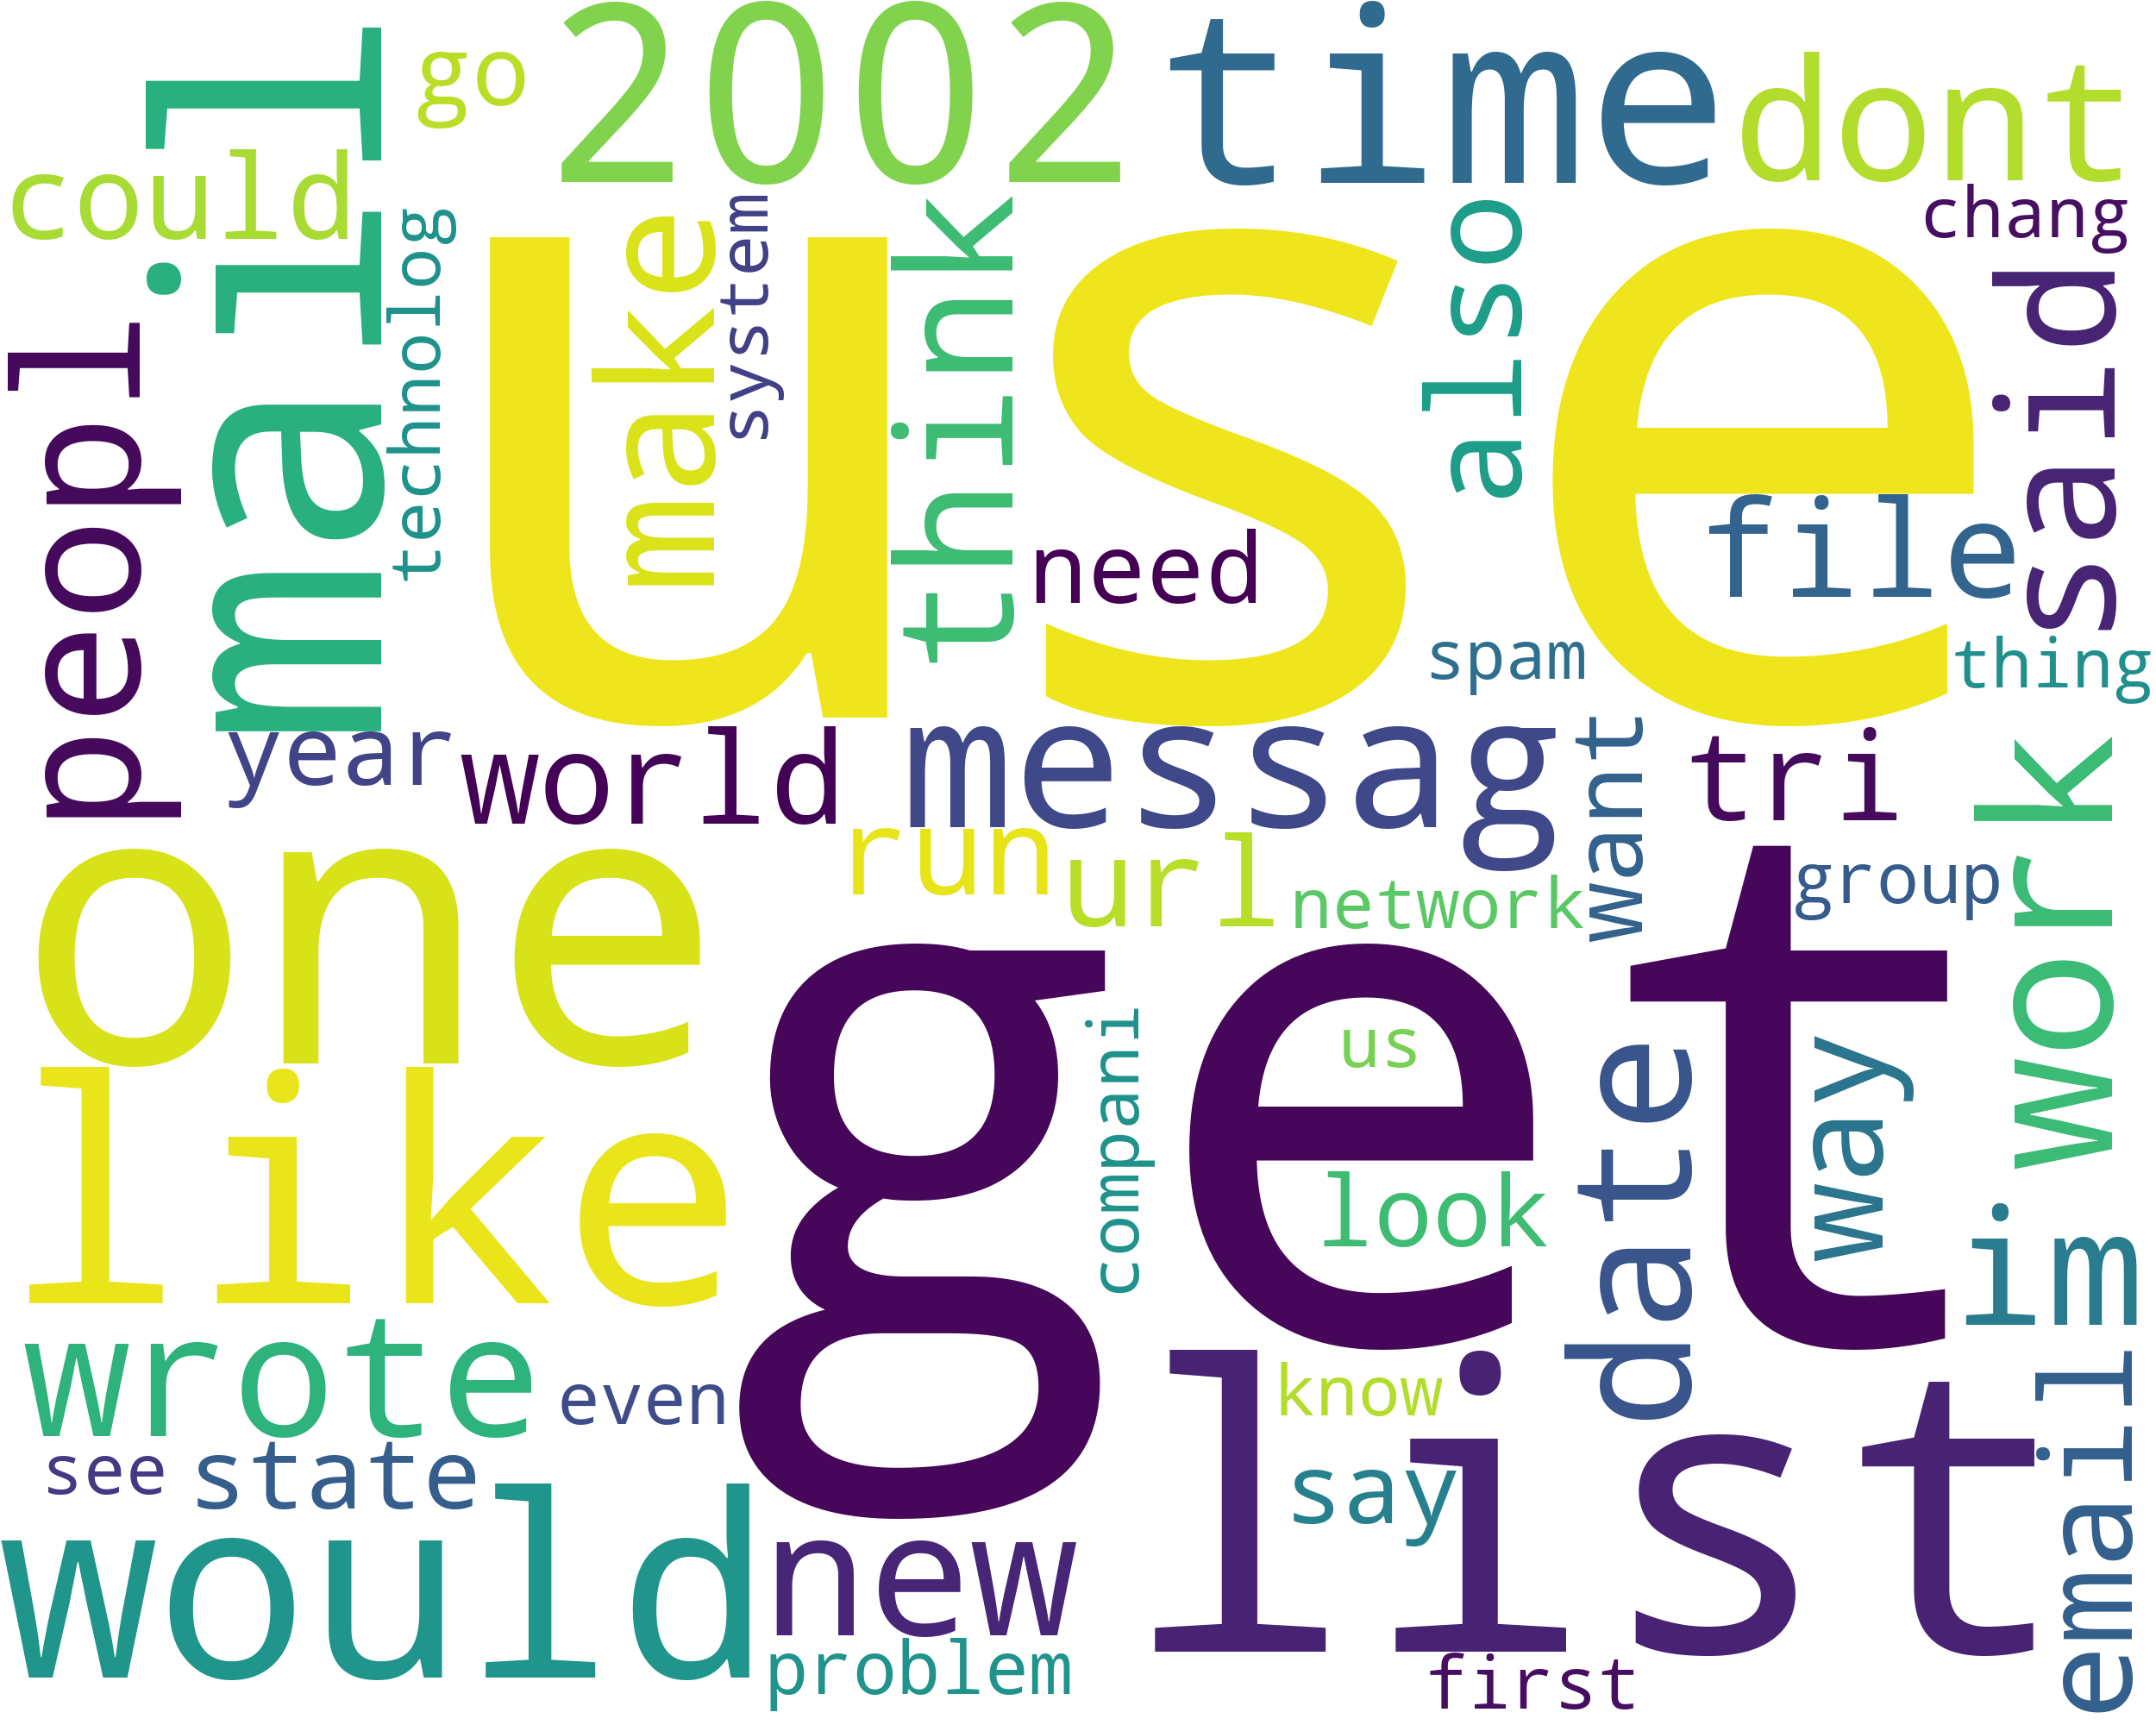
\includegraphics[width=\textwidth]{figures/ham_wc}
                \captionof{figure}{Ham}\label{fig:ham_wc}
             \end{minipage}

             Figures \ref{fig:spam_wc} and \ref{fig:ham_wc} show
             the most prominent 50 words in the corpus. Most the the words in the
             ham word cloud relate to business operations asking someone to do about
             task or getting times and dates of events. When you look at the spam
             word cloud you see a few similar words such as ``mail'' or ``get''.
             But in general you see words that you would associate with someone trying
             to get you to send them money or buy a product. Words like ``money'',
             ``offer'' and ``order'' are the epitome of this.
        
        \section{Classifier Selection}
        
            We selected various classifiers from the scikit-learn Python library. The 
            classifiers chosen for evaluation were Random Forest, K-Nearest Neighbors (KNN), 
            Support Vector Machine (SVM) with the radial basis function (RBF) kernel, and Bernoulli 
            Naive Bayes. All were chosen because they are well-known supervised machine learning 
            algorithms and generally good for classification tasks. 
        
        \section{Classifier Tuning}
            Once the classifiers were selected, we tuned them using a grid search with 5-fold 
            cross-validation maximizing accuracy. The parameters evaluated for each classifier along 
            with the chosen classifier parameters are as follows:
            
            \noindent\textbf{Random Forest}
            \begin{itemize}
                \setlength\itemsep{0em}
                \item Number of Estimators: 40
                \item Maximum Tree Depth: 40
            \end{itemize}
            \textbf{K-Nearest Neighbors}
            \begin{itemize}
                \setlength\itemsep{0em}
                \item Number of Neighbors: 10
                \item Weight by Distance?: Yes
            \end{itemize}
            \textbf{SVM}
            \begin{itemize}
                \setlength\itemsep{0em}
                \item Error Penalty: 10
                \item RBF Kernel Coefficient: 0.001
            \end{itemize}
            \textbf{Bernoulli Naive Bayes}
            \begin{itemize}
                \setlength\itemsep{0em}
                \item Learn Prior Probabilities?: No
                \item Smoothing?: None
            \end{itemize}

            We also examined the effect of tuning the number of feature words chosen by the TF-IDF 
            extractor. The number of feature words chosen for initial analysis was 50, but subsequent 
            tests ranged from 50 to 1050 in steps of 200.
        \section{Results}
            Classifiers were evaluated on precision and recall on the spam class. Overall, precision is
            weighted more heavily than recall in the evaluation because it would likely be more disruptive 
            to classify a ham email as spam than to let in an occasional spam message. Subsequently, the 
            classifiers were also subjected to various feature word counts to observe the effect.
            \subsection{General Precision and Recall}
                Overall, the classifiers performed well with just features extracted from the email body.
                Precision and recall comparison can be found in \autoref{fig:precision_recall} with direct 
                number comparison in \autoref{tab:precision_recall}. 

                \begin{Figure}
                    \begin{tabular}{|l|l|l|}
                        \hline
                        & Precision & Recall \\ \hline
                        KNN                                 & 90.91     & 51.02  \\ \hline
                        Naive Bayes                         & 83.67     & 83.67  \\ \hline
                        Random Forest                       & 98.84     & 86.73  \\ \hline
                        SVM                                 & 83.33     & 40.82  \\ \hline
                        Naive Bayes \cite{hovold2005naive}  & 98.46     & 99.66  \\ \hline
                        DBM \cite{tzortzis2007deep}         & 96.40     & 95.51  \\ \hline
                        SVM \cite{tzortzis2007deep}         & 96.14     & 95.24  \\ \hline
                    \end{tabular}
                    \captionof{table}{Precison and Recall}
                    \label{tab:precision_recall}
                \end{Figure}

                \begin{Figure}
                    \centering
                    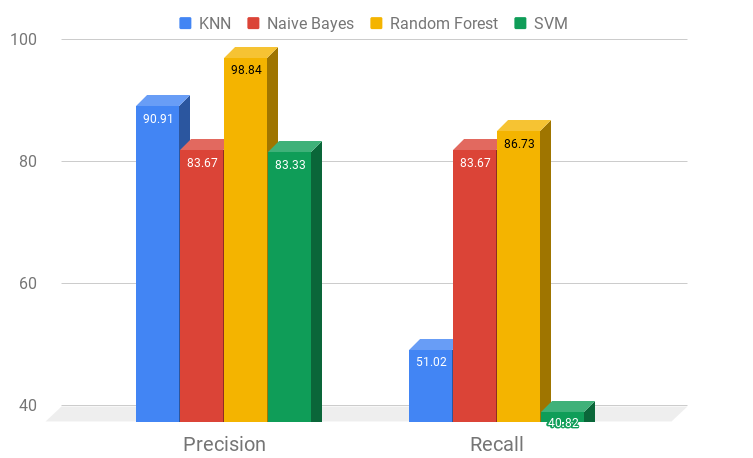
\includegraphics[width=\linewidth]{figures/precision_recall.png}
                    \captionof{figure}{Precison and Recall Comparison}
                    \label{fig:precision_recall}
                \end{Figure}

                While all classifiers had a precision greater than 80\%, the recall clearly divides the 
                classifiers into two groups. Those with over 80\% recall were Random Forest and Naive Bayes, 
                while the KNN and SVM both had a recall lower than 50\%. 
                
                Overall, the Random Forest classifier performed the best under our evaluation criteria 
                with an almost perfect precision. In fact, only one ham instance was misclassified as spam. 
                Random Forest also performed best on recall. The Naive Bayes classifier performed second best 
                with an even recall and precision.

                Comparing with classifiers by other researchers in \autoref{tab:precision_recall}, the 
                Random Forest classifier performs better in precision than all three classifiers by other researchers. 
                Looking at recall, however, leaves much to be desired. Likely due to focusing solely on email body 
                content for text analysis, our implementation misses important information in subject lines or 
                email addresses.


            \subsection{Effect of Number of Feature Words} 
                When increasing the number of feature words, precision increased dramatically for some classifiers. 
                Specifically, Naive Bayes and the SVM gained a precision increase of 10\% and 8\% respectively (See \autoref{fig:precision_word_effect}).
                However, the number of feature words did not seem to effect recall as much as precision (See \autoref{fig:recall_word_effect}).
                Only one classifier gained over 3\% precision from 50 feature words. Naive Bayes gained 10\% recall when increasing 
                the number of feature words from 50 to 250. This gain dropped off as the number of feature words increased.

                \begin{Figure}
                    \centering
                    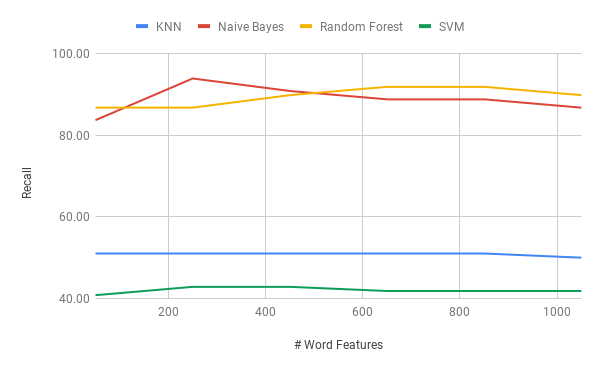
\includegraphics[width=\linewidth]{figures/recall_wv_effect.png}
                    \captionof{figure}{Effect of the number of feature words on classifier recall}
                    \label{fig:recall_word_effect}
                \end{Figure}
                
                \begin{Figure}
                    \centering
                    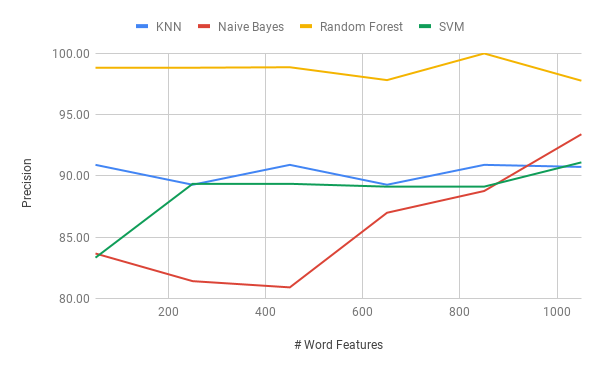
\includegraphics[width=\linewidth]{figures/precision_wv_effect.png}
                    \captionof{figure}{Effect of the number of feature words on classifier precision}
                    \label{fig:precision_word_effect}
                \end{Figure}

                Interestingly, Naive Bayes dropped in precision by over 2\% 
                for 250 and 450 feature words before having the largest gain of any classifier. 
                Possibly, the gain in recall had a negative effect on the precision.
                
        \section{Conclusion}

            This paper has shown that the usage of machine learning alone on email body text 
            along with a few other features can perform the spam classification task well. 
            However, our metrics are lower
            than the other papers we are comparing against ourselves. Adding more features
            that aren't word based may help even more with performance and also increasing the
            size of the dataset would help as well. We also recognize the limitations of
            this implementation lending itself to only classify emails from the early 2000s, as
            we did no testing on modern email data which may have a distribution that doesn't
            work well with our implementation.
        \nocite{*}
        \bibliography{paper} 
        \bibliographystyle{alpha}
    \end{multicols}
\end{document}